\documentclass[border={0.1cm 0.1cm 0.1cm 0.1cm}]{standalone}  %E,S,W,N

\usepackage{amssymb}
\usepackage{amsmath}
\usepackage{tikz}

\begin{document}
	
	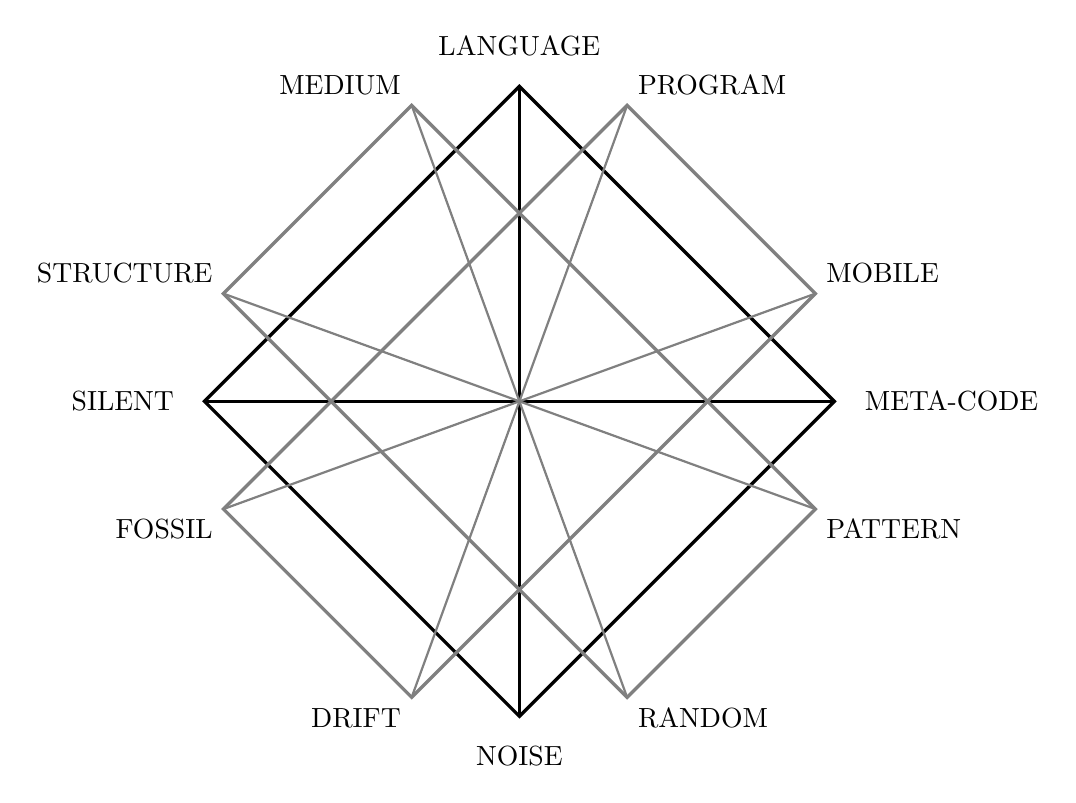
\begin{tikzpicture}[very thick]
	\def\s{4}	%size of square
	\def\r{20}	%steepness of rectangle
	
	%MAIN SQUARE
	\draw (0,\s)--(\s,0)--(0,-\s)--(-\s,0)--cycle;
	\draw (0,\s)--(0,-\s);	\draw (\s,0)--(-\s,0);
	
	%RECTANGLES
	\draw[gray] ({\s*cos(90-\r)},{\s*sin(90-\r)})--({\s*cos(0+\r)},{\s*sin(0+\r)})--({\s*cos(270-\r)},{\s*sin(270-\r)})--({\s*cos(180+\r)},{\s*sin(180+\r)})--cycle; %NE--SW
	\draw[gray] ({\s*cos(90+\r)},{\s*sin(90+\r)})--({\s*cos(180-\r)},{\s*sin(180-\r)})--({\s*cos(270+\r)},{\s*sin(270+\r)})--({\s*cos(0-\r)},{\s*sin(0-\r)})--cycle;
	%
	\foreach \i in {90-\r,0+\r,0-\r,270+\r}{
		\draw[gray,thick] ({\s*cos(\i)},{\s*sin(\i)})--(0,0);
		\draw[gray,thick] ({\s*cos(\i+180)},{\s*sin(\i+180)})--(0,0);
	}
	
	%LABELS
	\node[above] at ({(\s+0.25)*cos(90)}, {(\s+0.25)*sin(90)})  {LANGUAGE};
	\node[right] at ({(\s+0.25)*cos(00)}, {(\s+0.25)*sin(00)})  {META-CODE};
	\node[below] at ({(\s+0.25)*cos(-90)},{(\s+0.25)*sin(-90)}) {NOISE};
	\node[left]  at ({(\s+0.25)*cos(180)},{(\s+0.25)*sin(180)}) {SILENT};
	%
	\node[above right] at ({\s*cos(90-\r)},{\s*sin(90-\r)})   {PROGRAM};
	\node[above right] at ({\s*cos(0+\r)},{\s*sin(0+\r)})     {MOBILE};
	\node[below right] at ({\s*cos(-90+\r)},{\s*sin(-90+\r)}) {RANDOM};
	\node[below right] at ({\s*cos(0-\r)},{\s*sin(0-\r)})     {PATTERN};
	%
	\node[above left] at ({\s*cos(90+\r)},{\s*sin(90+\r)})   {MEDIUM};
	\node[above left] at ({\s*cos(180-\r)},{\s*sin(180-\r)}) {STRUCTURE};
	\node[below left] at ({\s*cos(180+\r)},{\s*sin(180+\r)}) {FOSSIL};
	\node[below left] at ({\s*cos(-90-\r)},{\s*sin(-90-\r)}) {DRIFT};
	\end{tikzpicture}
	
\end{document}